\documentclass[]{article}

\usepackage[dvipsnames]{xcolor}
\usepackage[landscape,margin=1cm]{geometry}
\usepackage{multicol}
\usepackage{graphicx}
\usepackage{amsmath}
\pagestyle{empty}

\begin{document}
\begin{multicols}{3}
\section{Courbes de Bézier}
\begin{center}
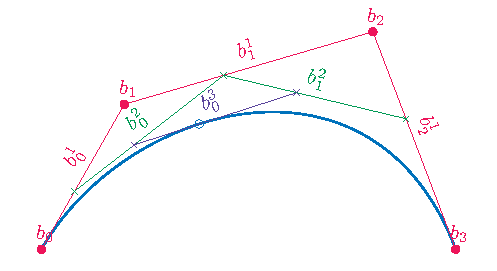
\includegraphics[width=0.6\columnwidth,page=1]{drwg_0.pdf}
\end{center}
\subsection{Triangle de Pascal}
\begin{center}
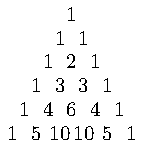
\includegraphics[scale=1,page=1]{drwg_1.pdf}
\end{center}
$$(a+b)^3=a^3+3a^2b+3ab^2+b^3$$
$$(a+b)^n=\sum_{k=0}^{n}\begin{pmatrix}
n\\k
\end{pmatrix}x^ky^{n-k}$$

$$\begin{pmatrix}
n\\ k
\end{pmatrix}=C^{n}_{k}=\frac{n!}{k!(n-k)!}$$
\subsection{Polynômes de Bernstein}
$$B_{i}^{m}(t)=\begin{pmatrix}m\\i\end{pmatrix}t^{i}(1-t)^{m-i}$$

\end{multicols}
\end{document}